\documentclass[11pt, a4paper]{article}

% ── Packages ──────────────────────────────────────────────
\usepackage[utf8]{inputenc}
\usepackage[T1]{fontenc}
\usepackage{lmodern}
\usepackage[margin=1in]{geometry}
\usepackage{amsmath, amssymb}
\usepackage{graphicx}
\usepackage{xcolor}
\usepackage{listings}
\usepackage{booktabs}
\usepackage{hyperref}
\usepackage{caption}
\usepackage{float}
\usepackage{enumitem}
\usepackage{microtype}
\usepackage{fancyhdr}
\usepackage{titlesec}
\usepackage{tcolorbox}

% ── Colours ───────────────────────────────────────────────
\definecolor{codegreen}{rgb}{0.25, 0.50, 0.35}
\definecolor{codegray}{rgb}{0.50, 0.50, 0.50}
\definecolor{codepurple}{rgb}{0.58, 0.00, 0.82}
\definecolor{codeblue}{rgb}{0.13, 0.29, 0.53}
\definecolor{backcolour}{rgb}{0.97, 0.97, 0.97}
\definecolor{accentred}{rgb}{0.75, 0.12, 0.12}

% ── Code listing style (Julia) ───────────────────────────
\lstdefinestyle{juliastyle}{
    backgroundcolor=\color{backcolour},
    commentstyle=\color{codegreen}\itshape,
    keywordstyle=\color{codeblue}\bfseries,
    numberstyle=\tiny\color{codegray},
    stringstyle=\color{accentred},
    basicstyle=\ttfamily\small,
    breakatwhitespace=false,
    breaklines=true,
    captionpos=b,
    keepspaces=true,
    numbers=left,
    numbersep=8pt,
    showspaces=false,
    showstringspaces=false,
    showtabs=false,
    tabsize=4,
    frame=single,
    rulecolor=\color{codegray!40},
    framesep=4pt,
    xleftmargin=18pt,
    framexleftmargin=18pt,
    morekeywords={function, end, if, elseif, else, return, using, for, in, true, false, nothing},
    literate=
      {μₛ}{{$\mu_s$}}2
      {μₖ}{{$\mu_k$}}2
      {fₛ}{{$f_s$}}2
      {fₖ}{{$f_k$}}2
      {≤}{{$\leq$}}1
      {≥}{{$\geq$}}1,
}
\lstset{style=juliastyle}

% ── Section styling ───────────────────────────────────────
\titleformat{\section}
  {\Large\bfseries\color{codeblue}}{\thesection}{1em}{}
\titleformat{\subsection}
  {\large\bfseries\color{codeblue!80}}{\thesubsection}{1em}{}

% ── Hyperlinks ────────────────────────────────────────────
\hypersetup{
    colorlinks=true,
    linkcolor=codeblue,
    urlcolor=accentred,
    citecolor=codegreen,
}

% ── Header/footer ─────────────────────────────────────────
\pagestyle{fancy}
\fancyhf{}
\fancyhead[L]{\small\textit{Friction, Force Pulses, and the Art of Piecewise ODEs}}
\fancyhead[R]{\small\thepage}
\renewcommand{\headrulewidth}{0.4pt}

% ── Custom commands ───────────────────────────────────────
\newcommand{\dd}[2]{\frac{d #1}{d #2}}
\newcommand{\ddd}[2]{\frac{d^2 #1}{d #2^2}}

% ══════════════════════════════════════════════════════════
\begin{document}

% ── Title ─────────────────────────────────────────────────
\begin{center}
    {\LARGE\bfseries Friction, Force Pulses, and the Art of Piecewise ODEs}\\[6pt]
    {\Large\color{codegray} A Block on a Rough Surface Under a Triangular Impulse}\\[20pt]
    {\large Claude Opus 4.6}\\[4pt]
    {\color{codegray}\today}
\end{center}

\vspace{8pt}
\noindent\rule{\textwidth}{0.5pt}

% ── Abstract ──────────────────────────────────────────────
\begin{abstract}
\noindent
A block of mass $m$ sits at rest on a rough horizontal surface.
A single symmetric triangular force pulse is applied, peaking above the
static friction threshold.  We derive the piecewise ODE governing
the block's motion, identifying the critical times for onset of sliding,
transition from acceleration to deceleration, and eventual re-sticking.
The system is then solved numerically using Julia's \texttt{OrdinaryDiffEq.jl}
package, producing time histories of force, velocity, and position.
The problem is an instructive example of a hybrid dynamical system ---
continuous dynamics interrupted by discrete state transitions --- where
the physics is exact and piecewise-linear, but the stick-slip friction
model demands care in numerical implementation.
\end{abstract}

\vspace{6pt}

\begin{quote}
\itshape
``Friction is the only force in classical mechanics that makes
physicists uncomfortable.  It is phenomenological, irreversible,
and full of surprises.''
\end{quote}

\vspace{4pt}

% ══════════════════════════════════════════════════════════
\section{A block, a surface, and a push}
\label{sec:setup}

Consider a block of mass $m$ sitting at rest on a rough horizontal surface.
The surface exerts two contact forces on the block: a normal force $N = mg$
(balancing gravity) and a friction force $f$ that opposes any tendency to slide.

Starting at $t = 1$\;s, we apply a horizontal force $F(t)$ shaped as a
single symmetric triangular pulse, peaking at $t = 3$\;s and vanishing
at $t = 5$\;s.  The peak force $F_{\max}$ exceeds the maximum static friction
$f_s = \mu_s mg$.  We seek $x(t)$, the position of the block.

\begin{tcolorbox}[colback=blue!5, colframe=blue!50!black, title=Physical System]
\begin{itemize}[itemsep=3pt]
    \item Mass: $m$
    \item Coefficients of friction: $\mu_s$ (static), $\mu_k$ (kinetic), with $\mu_k < \mu_s$
    \item Gravitational acceleration: $g$
    \item Peak applied force: $F_{\max} > \mu_s m g$
    \item Pulse timing: starts at $t = 1$, peaks at $t = 3$, ends at $t = 5$ (seconds)
\end{itemize}
\end{tcolorbox}

% ══════════════════════════════════════════════════════════
\section{The triangular pulse}
\label{sec:force}

The applied force rises linearly from $0$ to $F_{\max}$ over $[1, 3]$,
then falls linearly from $F_{\max}$ to $0$ over $[3, 5]$:

\begin{equation}
\boxed{
F(t) =
\begin{cases}
0 & t < 1 \\[4pt]
\displaystyle F_{\max}\,\frac{t - 1}{2} & 1 \le t \le 3 \\[8pt]
\displaystyle F_{\max}\,\frac{5 - t}{2} & 3 < t \le 5 \\[4pt]
0 & t > 5
\end{cases}
}
\label{eq:Ft}
\end{equation}

\noindent
Note that $F(1) = 0$, $F(3) = F_{\max}$, $F(5) = 0$, and the pulse is
symmetric about $t = 3$.  The impulse delivered is the area under the triangle:
$J = \tfrac{1}{2} \cdot F_{\max} \cdot 4 = 2\,F_{\max}$ (in N$\cdot$s).

% ══════════════════════════════════════════════════════════
\section{Two flavours of friction}
\label{sec:friction}

Friction in this problem has two distinct personalities.

\medskip
\noindent
\textbf{Static friction} (block at rest, $v = 0$): friction is \emph{reactive} ---
it exactly balances the applied force, up to a maximum:
\begin{equation}
f = F(t) \quad \text{provided } |F(t)| \le \mu_s m g.
\label{eq:static}
\end{equation}
The block does not move.  Static friction is a \emph{constraint}, not a
fixed force --- it gives only what is needed.

\medskip
\noindent
\textbf{Kinetic friction} (block sliding, $v > 0$): friction snaps to a fixed
value opposing the direction of motion:
\begin{equation}
f = \mu_k m g.
\label{eq:kinetic}
\end{equation}

\noindent
The discontinuous jump from $\mu_s mg$ to $\mu_k mg$ at the onset of motion
is the signature of Coulomb friction.  It is this jump that makes the problem
a \textbf{hybrid dynamical system}: continuous dynamics within each regime,
discrete switching between them.

% ══════════════════════════════════════════════════════════
\section{Critical times: when things change}
\label{sec:critical}

\subsection{Onset of motion: $t = t_1$}

The block begins to slide when $F(t)$ first exceeds the static friction limit.
During the rising phase ($1 \le t \le 3$):
\begin{equation}
F(t_1) = \mu_s m g
\qquad\Longrightarrow\qquad
F_{\max}\,\frac{t_1 - 1}{2} = \mu_s m g
\end{equation}

\begin{equation}
\boxed{t_1 = 1 + \frac{2\,\mu_s m g}{F_{\max}}}
\label{eq:t1}
\end{equation}

\noindent
Since $F_{\max} > \mu_s m g$, we have $1 < t_1 < 3$: the block always
starts moving during the rising phase.

\subsection{Force drops below kinetic friction: $t = t_2$}

Once sliding, friction is only $\mu_k m g$.  The net force becomes zero
when $F(t) = \mu_k m g$ on the \emph{falling} side of the pulse:
\begin{equation}
F_{\max}\,\frac{5 - t_2}{2} = \mu_k m g
\end{equation}

\begin{equation}
\boxed{t_2 = 5 - \frac{2\,\mu_k m g}{F_{\max}}}
\label{eq:t2}
\end{equation}

\noindent
For $t > t_2$, the applied force is insufficient to overcome kinetic friction,
and the block decelerates.  The fact that $t_2 > 3$ (the peak) --- typically
well past it --- means the block continues \emph{accelerating} long after the
force has begun to decline.  Momentum accumulates silently.

% ══════════════════════════════════════════════════════════
\section{The four phases of motion}
\label{sec:phases}

The dynamics splits cleanly into four regimes.

\begin{table}[H]
\centering
\caption{Phases of motion under the triangular pulse.  Each phase has a
         different governing ODE due to the stick-slip transition and
         the piecewise force.}
\label{tab:phases}
\begin{tabular}{@{}clll@{}}
\toprule
\textbf{Phase} & \textbf{Time interval} & \textbf{Physics} & \textbf{Net acceleration} \\
\midrule
I   & $0 \le t < t_1$     & Static equilibrium     & $\ddot{x} = 0$ \\[3pt]
II  & $t_1 \le t \le 3$   & Sliding, force rising   & $\ddot{x} = \frac{F_{\max}}{2m}(t-1) - \mu_k g$ \\[3pt]
III & $3 < t \le t_2$     & Sliding, force falling  & $\ddot{x} = \frac{F_{\max}}{2m}(5-t) - \mu_k g$ \\[3pt]
IV  & $t > t_2$           & Friction braking        & $\ddot{x} = \frac{F_{\max}}{2m}(5-t) - \mu_k g$ \\
\bottomrule
\end{tabular}
\end{table}

\noindent
Phase~IV deserves a comment.  For $t_2 < t \le 5$, the applied force is still
present but insufficient; for $t > 5$, it vanishes entirely and the ODE becomes
simply $\ddot{x} = -\mu_k g$.  In both sub-phases, the block decelerates.

% ══════════════════════════════════════════════════════════
\section{The governing ODE}
\label{sec:ode}

Newton's second law in the horizontal direction gives the complete,
piecewise equation of motion:

\begin{tcolorbox}[colback=accentred!5, colframe=accentred!70!black, title=Master Equation of Motion]
\begin{equation}
\boxed{
m\,\ddot{x} =
\begin{cases}
0 & 0 \le t < t_1 \;\text{(static equilibrium)} \\[6pt]
\displaystyle \frac{F_{\max}}{2}(t-1) - \mu_k m g & t_1 \le t \le 3 \;\text{(sliding, force rising)} \\[8pt]
\displaystyle \frac{F_{\max}}{2}(5-t) - \mu_k m g & 3 < t \le 5 \;\text{(sliding, force falling)} \\[8pt]
-\mu_k m g & t > 5 \;\text{(friction braking)}
\end{cases}
}
\label{eq:master}
\end{equation}

\medskip
\noindent
\textbf{Subject to:} \;$x(0) = x_0$, $\;\dot{x}(0) = 0$, and the
re-sticking constraint $\dot{x} \to 0^+ \;\wedge\; F(t) \le \mu_s mg
\;\Rightarrow\;$ block returns to static equilibrium.
\end{tcolorbox}

\subsection{Closed-form solutions by phase}

Since each phase has a linear (or constant) acceleration, the velocity
and position are polynomials in $t$, joined by continuity conditions.

\medskip
\noindent
\textbf{Phase~II} ($t_1 \le t \le 3$): with $v(t_1) = 0$,
\begin{align}
v(t) &= \frac{F_{\max}}{4m}\left[(t-1)^2 - (t_1-1)^2\right] - \mu_k g\,(t - t_1)
\label{eq:v_phase2} \\[6pt]
x(t) &= x_0 + \frac{F_{\max}}{4m}\left[\frac{(t-1)^3 - (t_1-1)^3}{3} - (t_1-1)^2(t - t_1)\right] - \frac{\mu_k g}{2}(t - t_1)^2
\label{eq:x_phase2}
\end{align}

\medskip
\noindent
\textbf{Phase~III} ($3 < t \le t_2$): with $v(3) = v_3$, $x(3) = x_3$
from Phase~II,
\begin{align}
v(t) &= v_3 - \frac{F_{\max}}{4m}\left[(5-t)^2 - 4\right] - \mu_k g\,(t - 3)
\label{eq:v_phase3} \\[6pt]
x(t) &= x_3 + v_3(t-3) + \frac{F_{\max}}{4m}\left[\frac{(5-t)^3 - 8}{3} + 4(t-3)\right] - \frac{\mu_k g}{2}(t-3)^2
\label{eq:x_phase3}
\end{align}

\medskip
\noindent
\textbf{Phase~IV} ($t > 5$): pure friction braking with $v(5) = v_5$,
\begin{equation}
v(t) = v_5 - \mu_k g\,(t - 5), \qquad
t_{\text{stop}} = 5 + \frac{v_5}{\mu_k g}
\label{eq:tstop}
\end{equation}

% ══════════════════════════════════════════════════════════
\section{Dimensionless form}
\label{sec:dimless}

Define $\hat{t} = (t - 1)/2$ so that the pulse occupies $\hat{t} \in [0, 2]$
with peak at $\hat{t} = 1$.  The two dimensionless parameters that control
everything are:
\begin{equation}
\boxed{
\alpha = \frac{\mu_s m g}{F_{\max}} \quad (\text{static friction ratio}),
\qquad
\beta = \frac{\mu_k m g}{F_{\max}} \quad (\text{kinetic friction ratio})
}
\label{eq:dimless_params}
\end{equation}

\noindent
The problem requires $\alpha < 1$ (peak exceeds static friction) and
$\beta < \alpha$ (kinetic $<$ static).  The dimensionless ODE for
$\hat{t} > \alpha$ (the onset time) is simply:
\begin{equation}
\boxed{\ddd{\hat{x}}{\hat{t}} = \hat{F}(\hat{t}) - \beta}
\label{eq:dimless_ode}
\end{equation}
where $\hat{F}(\hat{t}) = \hat{t}$ for $0 \le \hat{t} \le 1$ and
$\hat{F}(\hat{t}) = 2 - \hat{t}$ for $1 < \hat{t} \le 2$.
All the physics lives in $\alpha$ and $\beta$.

% ══════════════════════════════════════════════════════════
\section{Enter Julia}
\label{sec:julia}

We convert the second-order ODE~\eqref{eq:master} into a first-order system
by defining $u_1 = x$ (position) and $u_2 = v$ (velocity):
\begin{equation}
\begin{cases}
\;\dot{u}_1 = u_2 \\[6pt]
\;\dot{u}_2 = \bigl[F(t) - \mu_k m g\bigr] / m \quad \text{(sliding)} \\[4pt]
\;\dot{u}_1 = \dot{u}_2 = 0 \quad\qquad\qquad\;\;\; \text{(stuck)}
\end{cases}
\label{eq:system}
\end{equation}

\noindent
The stick-slip logic enters the right-hand side as a conditional branch:
if $v \le 0$ and $F(t) \le \mu_s mg$, the block is stuck and both derivatives
are zero.  Otherwise, kinetic friction applies.

\subsection{The triangular pulse in code}

\begin{lstlisting}[caption={Triangular force pulse. Returns zero outside
  $[1, 5]$, ramps linearly to \texttt{Fmax} at $t = 3$.}]
function F_pulse(t, Fmax)
    if t < 1.0
        return 0.0
    elseif t ≤ 3.0
        return Fmax * (t - 1.0) / 2.0
    elseif t ≤ 5.0
        return Fmax * (5.0 - t) / 2.0
    else
        return 0.0
    end
end
\end{lstlisting}

\subsection{The right-hand side with stick-slip logic}

\begin{lstlisting}[caption={In-place RHS function for
  \texttt{OrdinaryDiffEq.jl}.  The conditional branch encodes
  the static/kinetic friction transition.}]
function f!(du, u, p, t)
    m, μₛ, μₖ, g, Fmax = p

    x = u[1]   # position
    v = u[2]   # velocity

    F = F_pulse(t, Fmax)
    fₛ = μₛ * m * g   # max static friction
    fₖ = μₖ * m * g   # kinetic friction

    if v ≤ 0.0 && F ≤ fₛ
        # Stuck: static friction balances applied force
        du[1] = 0.0
        du[2] = 0.0
    else
        # Sliding: kinetic friction opposes motion
        du[1] = v
        du[2] = (F - fₖ) / m
    end
end
\end{lstlisting}

\subsection{Problem definition and solve}

\begin{lstlisting}[caption={Setting up and solving the ODE.  The key
  subtlety: \texttt{tstops} forces the adaptive integrator to step
  at force discontinuities, and \texttt{dtmax} prevents it from
  leaping over the stick-slip transition.}]
using OrdinaryDiffEq

u0 = [0.0, 0.0]   # [x0, v0]
tspan = (0.0, 8.0)
p = [2.0, 0.5, 0.3, 9.81, 15.0]   # m, μₛ, μₖ, g, Fmax

prob = ODEProblem(f!, u0, tspan, p)
sol = solve(prob, Tsit5(),
            tstops=[1.0, 3.0, 5.0], dtmax=0.01)
\end{lstlisting}

\noindent
The parameters used are listed in Table~\ref{tab:params}.

\begin{table}[H]
\centering
\caption{Numerical parameters for the simulation.}
\label{tab:params}
\begin{tabular}{@{}llll@{}}
\toprule
\textbf{Parameter} & \textbf{Symbol} & \textbf{Value} & \textbf{Units} \\
\midrule
Mass                    & $m$        & 2.0   & kg \\
Static friction coeff.  & $\mu_s$    & 0.5   & --- \\
Kinetic friction coeff. & $\mu_k$    & 0.3   & --- \\
Gravitational accel.    & $g$        & 9.81  & m/s$^2$ \\
Peak applied force      & $F_{\max}$ & 15.0  & N \\
\midrule
Static friction limit   & $\mu_s mg$ & 9.81  & N \\
Kinetic friction        & $\mu_k mg$ & 5.886 & N \\
Onset time              & $t_1$      & 2.308 & s \\
Deceleration onset      & $t_2$      & 4.215 & s \\
\bottomrule
\end{tabular}
\end{table}

\subsection{A numerical trap: the silent zero}

Without \texttt{tstops} and \texttt{dtmax}, the solver produces just 8 time
points and returns $x(8) = 0$ --- the block never moves.  What happened?

The RHS is identically $[0, 0]$ during the stuck phase.  The adaptive
Tsit5 stepper sees zero derivatives, concludes nothing is happening,
and takes an enormous step --- leaping from $t = 0$ to well past
$t = 5$ without ever evaluating $F(t)$ at a time where it exceeds
$\mu_s mg$.  The transition is invisible to the integrator.

This is a general hazard with switching ODEs: \emph{adaptive solvers can
step right over a discontinuity if the RHS is flat on both sides of it.}
The fix is to explicitly inform the solver of the switching times via
\texttt{tstops}, and to cap the step size with \texttt{dtmax} so it
cannot leap over the breakaway.

% ══════════════════════════════════════════════════════════
\section{Results}
\label{sec:results}

Figure~\ref{fig:results} shows the complete time history of the system.

\begin{figure}[H]
    \centering
    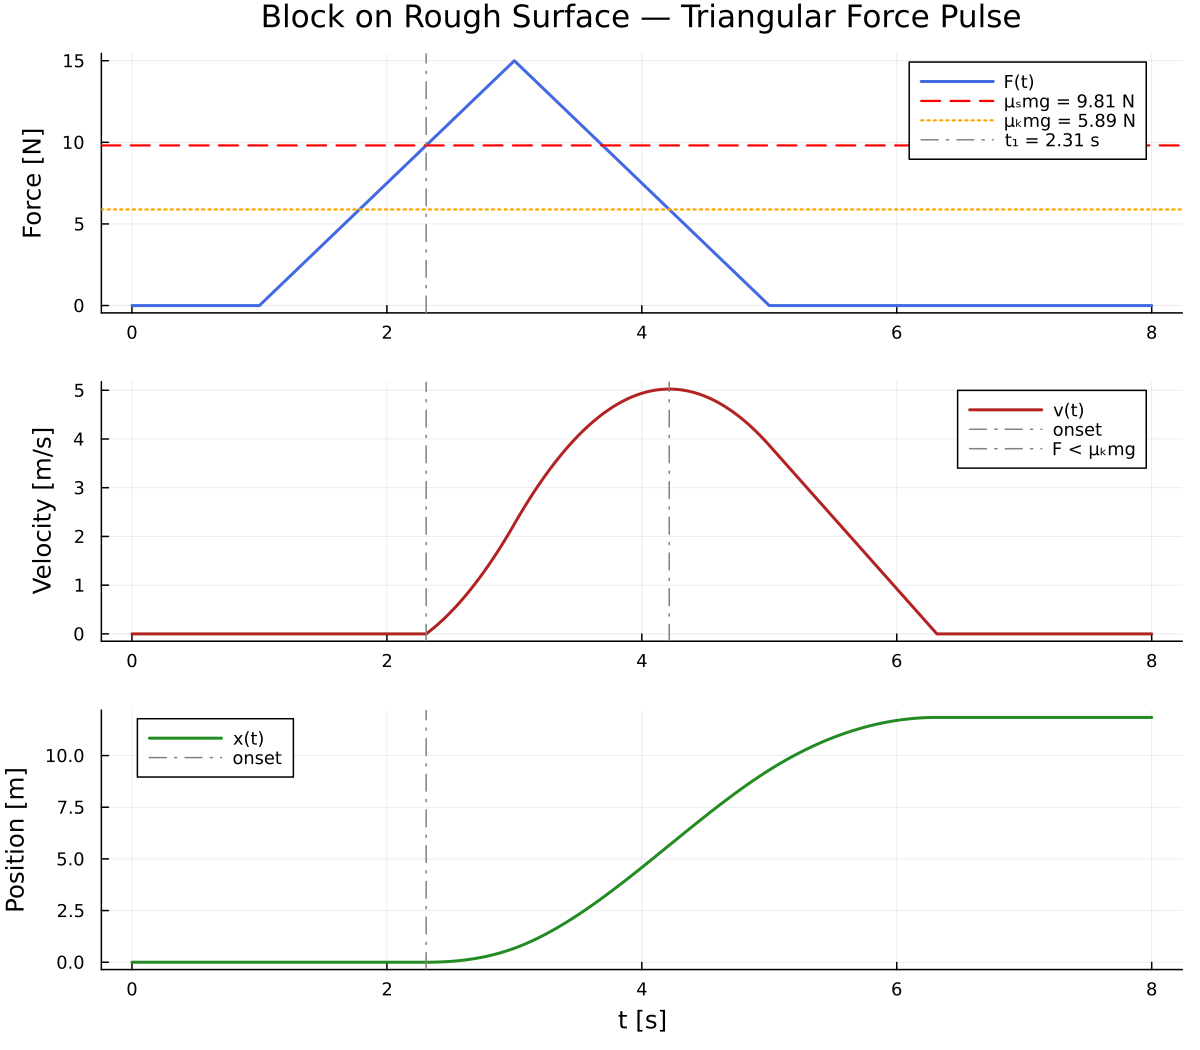
\includegraphics[width=\textwidth]{triangular_pulse_block.png}
    \caption{Three-panel time history of the block under a triangular
             force pulse.
             \textbf{Top:} Applied force $F(t)$ (blue) with the static
             friction limit $\mu_s mg = 9.81$\;N (red dashed) and
             kinetic friction $\mu_k mg = 5.89$\;N (orange dotted).
             The vertical line marks $t_1 = 2.31$\;s, when the block
             breaks free.
             \textbf{Middle:} Velocity $v(t)$.  The block accelerates
             from $t_1$ through the force peak at $t = 3$ and beyond,
             reaching maximum velocity near $t_2 = 4.22$\;s when the
             applied force drops below kinetic friction.  After $t = 5$,
             pure friction braking decelerates the block to rest.
             \textbf{Bottom:} Position $x(t)$.  The block slides a total
             of approximately $11.85$\;m before coming to rest.
             Solved with Tsit5 (814 time points).}
    \label{fig:results}
\end{figure}

\subsection{Reading the physics from the curves}

Several features of Figure~\ref{fig:results} deserve attention:

\begin{enumerate}[itemsep=4pt]
    \item \textbf{The block sits still for over 2 seconds.}  The force
          must ramp up from zero to $9.81$\;N before anything happens.
          During this time, static friction absorbs the applied force
          perfectly.

    \item \textbf{Peak velocity occurs after the force peak.}  The force
          peaks at $t = 3$, but the block keeps accelerating until
          $t_2 = 4.22$ --- more than a second later.  This is because
          kinetic friction ($5.89$\;N) is much less than the force
          at $t = 3$ ($15$\;N).  The applied force must drop
          significantly before friction wins.

    \item \textbf{The position curve is an asymmetric S.}  The long
          flat region (stuck), the steep rise (accelerating), and the
          gradual plateau (braking) reflect the three dynamical regimes.

    \item \textbf{Total displacement: $\sim$11.85\;m.}  For a 2\;kg
          block with $F_{\max} = 15$\;N and relatively low kinetic
          friction ($\mu_k = 0.3$), this is physically reasonable.
          The block accumulates substantial momentum during the nearly
          2 seconds of net positive acceleration.

    \item \textbf{The block comes cleanly to rest.}  The final velocity
          is $\sim 10^{-5}$\;m/s (numerical residual), confirming
          that the stick-slip logic correctly captures re-sticking.
\end{enumerate}

% ══════════════════════════════════════════════════════════
\section{The moral}
\label{sec:moral}

This problem is piecewise-linear --- every phase has a closed-form
solution as a polynomial in $t$.  And yet, it resists a careless
numerical approach.  The stick-slip transition, the kinks in the
force profile, and the dormant initial phase conspire to fool
adaptive integrators into missing the entire event.

The lesson is broader than this particular problem:

\medskip
\noindent
\textbf{Hybrid dynamics require hybrid thinking.}  A smooth ODE solver
is not enough when the physics has discrete transitions.  You must
tell the integrator where to look --- via \texttt{tstops}, callbacks,
or event detection --- or it will look right past the interesting part.

\medskip
\noindent
\textbf{The $\mu_s$--$\mu_k$ gap creates hysteresis.}  The block needs
$\mu_s mg$ to start, but once moving, friction drops to $\mu_k mg$.
This asymmetry means the block cannot re-stick until the velocity
reaches zero \emph{and} the applied force drops below $\mu_s mg$ ---
a condition rarely met during the pulse.  The gap between static and
kinetic friction is small on paper but large in its dynamical consequences.

\medskip
\noindent
\textbf{Dimensionless parameters reveal the structure.}  The entire
problem collapses to two numbers: $\alpha = \mu_s mg / F_{\max}$
and $\beta = \mu_k mg / F_{\max}$.  Every qualitative feature ---
how long the block sits still, how far past the peak it keeps
accelerating, how far it slides --- is controlled by these ratios.

\vfill

% ══════════════════════════════════════════════════════════
\begin{thebibliography}{9}

\bibitem{rackauckas}
C.~Rackauckas and Q.~Nie,
``DifferentialEquations.jl --- A Performant and Feature-Rich Ecosystem
for Solving Differential Equations in Julia,''
\textit{Journal of Open Research Software} \textbf{5}(1), 15 (2017).

\bibitem{tsitouras}
Ch.~Tsitouras,
``Runge--Kutta pairs of order 5(4) satisfying only the first column
simplifying assumption,''
\textit{Computers \& Mathematics with Applications} \textbf{62}(2),
770--775 (2011).

\bibitem{stewart}
D.~E.~Stewart,
``Rigid-body dynamics with friction and impact,''
\textit{SIAM Review} \textbf{42}(1), 3--39 (2000).

\end{thebibliography}

\vspace{12pt}
\begin{center}
    \small\color{codegray}
    All code and figures generated with Julia 1.x and \texttt{OrdinaryDiffEq.jl}.
\end{center}

\end{document}
